\chapter{Literature Study}
\label{chp:litreview}

With the project objectives in mind, we now present a study of the literature regarding autonomous racing.
We start this chapter with a review of existing approaches to designing autonomous driving algorithms.
A taxonomy of these approaches to solve the autonomous racing problem is shown in Figure \ref{fig:lit_tax_sec}.
We end the chapter with a discussion of the research gaps found in the literature, as well as a summary of the expected contributions of this project towards the literature.

\begin{figure}[htb!]
    \centering
    \input contents/chapt2/figs/literature_taxonomy_sections.tex
    \caption[A taxonomy of the autonomous racing literature with sections]{A taxonomy of approaches to solving the autonomous racing problem.}
    \label{fig:lit_tax_sec}
\end{figure}


\section{Classical approaches}\label{sec:classic}

% The classical approach is the traditional method of designing autonomous driving architectures.
% It is split into an \emph{offline} and \emph{online} phase, as shown in Figure \ref{fig:full_stack}.
% The offline phase occurs before the vehicle is deployed on the track.
% If the track is known, then a global trajectory (also known as a \emph{raceline}) can be computed during this offline phase.
% This raceline typically comprises a path ($x(t), y(t)$) and velocity profile $v(t)$ that extends along the entire track.

% In the online phase, the vehicle is deployed onto and allowed to interact with a simulated or real track.
% The concern during this phase is processing sensor input to generate control outputs.
% The classical approach to controlling the car during the online phase is to process the sensor data using a series of modules with well defined functions.
% This has the advantages that each function can be developed and improved independently of the others, and vehicle behaviour can easily be debugged.

% The modules most used by the classic pipeline are perception, local planning and control.
% Perception algorithms derive knowledge about the vehicles surroundings. 
% This includes constructing an updated map, localising the vehicle within that map, and detecting obstacles such as other vehicles. 
% Information from the perception module is passed onto the local planner and controller to generate and follow a trajectory  \cite{Betz2021}.
% Due to their relevance to  our project, methods for local planning and control are now discussed in more detail. 

% \begin{figure}[h]
%     \centering
%     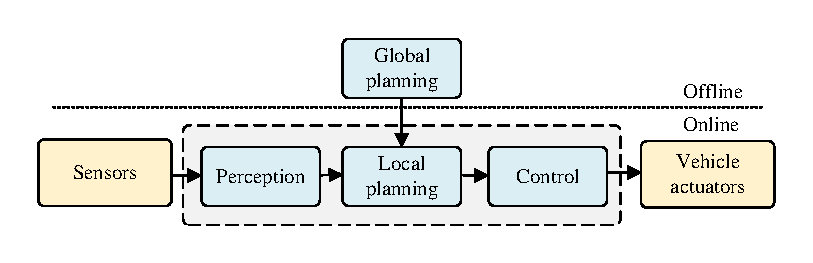
\includegraphics{contents/chapt2/figs/classic_pipeline.pdf}
%     \caption{The classic autonomous driving pipeline.}
%     \label{fig:full_stack}
% \end{figure}

Classical approaches split the task of generating actuator commands from sensor data into three distinct phases, namely (a) perception, (b) planning and (c) control \cite{Betz2021}.
This generic framework is illustrated in Figure \ref{fig:full_stack}.
Classical approaches have successfully been used to control full scale racing cars \cite{Valls2018, alvarez2022, Nekkah2020}, as well as small scaled racing cars \cite{Liniger2015}.
Methods for planning and control are studied with emphasis on techniques that are used to address the sim2real gap within classical systems.
However, perception algorithms are not discussed because they are outside of the scope for this project.

\begin{figure}[h]
    \centering
    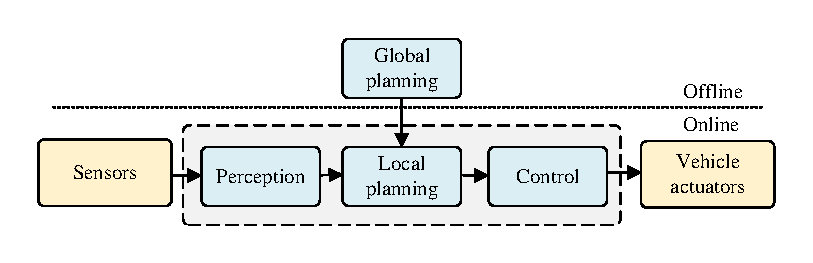
\includegraphics{contents/chapt2/figs/classic_pipeline.pdf}
    \caption{The classic autonomous driving pipeline.}
    \label{fig:full_stack}
\end{figure}

\subsection{Planning}
\label{sec:trajectory_planning}

Planning without a vehicle model
\cite{DalBianco2019, }
Approaches are efficient.
Furthermore, the computational burden of optimisation can be shifted to before the race begins.
However, these approaches do not directly address vehicle modelling error.






% The purpose of the local planner is to compute a trajectory based on the current information provided by the perception module.
% Local trajectory planning is a requirement for the safe deployment of racing vehicles because racing is a highly dynamic environment, especially when multiple vehicles are involved.
% This means that global path that was computed offline may be infeasible or unsafe due to changing conditions on the track.
% The challenge for local planners is then to compute a trajectory faster than real-time.

% Similar to the raceline, the local trajectory is comprised of a path and velocity profile, but with a finite horizon. 
% A finite horizon is used because optimising a trajectory over the entire track is computationally expensive, and also only the part of the trajectory immediately in front of the vehicle is relevant to the current control action.

% Model Predictive Control (MPC) methods are the most commonly used and state of the art methods for local planning \cite{Betz2021}. 
% This method relies on a vehicle dynamics model to optimise a finite horizon trajectory by minimising a specified cost function.
% Only the first section of the trajectory is executed before optimising again.
% The MPC method is powerful because it directly considers the vehicle and track constraints.
% Therefore, the trajectory generated is safe so long as these constraints specified correctly and the horizon of the trajectory long enough \cite{Schwenzer2021}.

% Despite achieving impressive results there are many challenges to deploying MPC for trajectory planning.
% A major drawback is that performing an optimisation at every time step is computationally expensive.
% As such, many applications of MPC in autonomous racing, such as that by  Anderson et al. \cite{Anderson2016} and Funke et al. \cite{Funke2017} utilise simplified linear dynamics models that do not entirely capture the full non-linear system dynamics.
% Furthermore, MPCs rely on convexification (such as with quadratic approximation) of the cost function to be optimised \cite{Williams2017}.


\subsection{Control}
\label{sec:control}

In the previous section, we described the common method of generating a local trajectory.
This local trajectory provides the reference information to compute control commands used to actuate the motors.
The goal of the controller is to minimise the error between the actual and planned trajectory.
By compensating for this error, controllers effectively absorb uncertainty from the system.
At this level of abstraction, the control commands are the steering angle $\delta$ for \emph{lateral} control, and longitudinal acceleration $a_{\text{long}}$ for \emph{longitudinal} control.
Lateral and longitudinal control are commonly decoupled and treated as separate problems:
while lateral controllers are used for path tracking, longitudinal controllers are used for velocity tracking.

\subsubsection*{Lateral Control}

Many of the approaches surveyed employed classic controllers that utilise well known principles in the fields of path and velocity tracking, namely feedforward and feedback control.
Feedback controllers compute control commands using the error between the actual and desired vehicle trajectory, whereas feedforward controllers are open-loop, calculating the control signal based only on the properties of the vehicle and desired path with no error compensation.

A basic feedback lateral controller for path tracking, known as pure pursuit, is presented by Coultier \cite{Coulter_1992}. 
Pure pursuit calculates the steering angle the car should maintain to reach a target point on the path which is a fixed distance away from the vehicle, under the assumption that the vehicle wheels do not slip. 
Despite this no-slipping assumption, the pure pursuit controller proved robust.
Other classic approaches such as that by Hoffman et al. \cite{Hoffmann2007}, utilise feedback controllers which compute a control signal based on the cross track and heading error.
These errors are the distance between the closest point on the path to the front axle of the vehicle, and the the angle between the heading of the vehicle and the tangent on the closest point on the path, respectively.

Ni and Hu \cite{Ni2017}, Fu et al. \cite{Fu2016} and Kritayakirana and Gerdes \cite{Kritayakirana2012} further the work by Hoffman et al. \cite{Hoffmann2007} by using both feedback and feedforward control. 
Their feedforward controllers use linearised vehicle dynamics models and information about the path to compute a desired steering angle. Feedback control is added to the value computed by the feedforward controller.
The desired behaviour of this controller setup is to imitates a human driver that computes a steering angle based on knowledge about the path and vehicle, then trims the steering angle based on the deviation from the intended path.

Besides classical control, MPCs are one of the main methods behind many autonomous racing controllers that have been implemented on physical vehicles.
Alvarez et al. \cite{alvarez2022} and Nekkah et al. \cite{Nekkah2020} develop MPCs for the lateral control of Formula Student racecars.
Their MPCs  are similar to those described in the trajectory planning section, as they use a linearised vehicle dynamics model to forecast a series of optimal series of states $\{ x_t, x_{t+1}, ..., x_{t+N}\}$ and corresponding actions $\{ u_t, u_{t+1}, ..., u_{t+N}\}$. 
The first control action $u_{t}$ then is executed and the optimisation process is run again.
However, reliance on an accurate vehicle dynamics model is a serious issue for MPC applied to the control setting. 
If an inaccurate vehicle model is used, the vehicle may deviate from its intended path.
Futhermore, model inaccuracies are likely to occur due to the difficulty of measuring the vehicle model parameters \cite{Kabzan2019, Pan2017}.

\subsubsection*{Longitudinal Control}
Longitudinal control for velocity tracking is simpler than path tracking, and is usually achieved using proportional integral derivative (PID) control. 
For instance, Nekkah et al. \cite{Nekkah2020} use a feedforward proportional integral (PI) controller for tracking a velocity target. 
In this case, feedforward control works because the longitudinal dynamics of the race car are known.
Other approaches, such as those by Hoffman et al. \cite{Hoffmann2007} and Alvarez et al. \cite{alvarez2022} utilise feedback proportional integral (PI) control to track a velocity target.

Ni and Hu \cite{Ni2017}, Fu et al. \cite{Fu2016} and Kritayakirana and Gerdes \cite{Kritayakirana2012} take control a step further by calculating the maximum allowable longitudinal acceleration before the tires slip.
This is done using a $g$-$g$ diagram that describes the friction limit of the tires in terms of lateral and longitudinal acceleration, 
%The curvature of the planned path is used to calculate the lateral acceleration, which in turn is used to estimate the maximum allowable longitudinal acceleration and velocity. 
allowing the vehicle to operate close to the tire friction limits.
The calculated velocity is then tracked with both feedforward and feedback control.

%In summary, the modularised pipeline adopted by classical approaches has eased the driving algorithm development process.
%By decoupling the tasks of perception, planning and control, research efforts into each task have achieved impressive results.
%Within the literature reviewed, many local planners and some controllers are based on MPC algorithms.
%The limitations to MPC include the requirement for expensive computation (especially for non-linear dynamic models), expensive sensor suites due to the need for frequent and accurate state information, and lack of flexibility in the cost function. 
%In particular, reliance on an accurate vehicle dynamics model is a serious issue due to the difficulty of measuring the vehicle model parameters \cite{Kabzan2019, Pan2017}.

%However, there are several robust classical controllers.


\section{End-to-end pipeline}
\label{sec:end_to_end}

The limitations of optimisation techniques from classical methods has led to research in learning-based systems that improve the vehicle dynamics model or action policy with real-world data and allow more complex cost formulations and non-linear dynamics \cite{Fuchs2021}.
Many learning approaches use an end-to-end pipeline whereby a single neural network predicts control outputs from sensor data, thus performing the task of the entire classical pipeline.
This end-to-end pipeline is illustrated in Figure \ref{fig:end_to_end}.
If the circuit is known beforehand (as is the case with the F1tenth competitions), then the neural network can be trained to complete a circuit lap in an offline manner using either generated training data (imitation learning) or simulated track interactions (reinforcement learning) before being deployed and allowed to interact with the real track.
We now present a summary of research efforts into the two paradigms by which the neural networks are trained (i.e., imitation learning and reinforcement learning).

\begin{figure}[htb!]
    \centering
    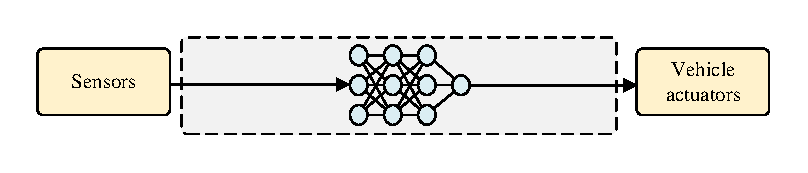
\includegraphics{contents/chapt1/figs/end_to_end.pdf}
    \caption{The end-to-end autonomous driving pipeline.}
    \label{fig:end_to_end}
\end{figure}

\subsection{Imitation learning}
\label{sec:imitation_learning}

Imitation learning techniques train a neural network to mimic an expert driver.
The process is analogous to supervised learning, where labelled data is used to train an algorithm to predict outcomes on new data.
In the context of autonomous racing, the labelled training data is produced by allowing an optimisation method or human to drive the vehicle.
This produces a set of control commands which act as the labels for the inputs to the neural network.
Supervised learning is then used to train an algorithm to predict control commands for new data.
Imitation learning is a good choice for training a neural network if it is feasible for an expert to demonstrate optimal behaviour \cite{Osa_2018}.

Many approaches, such as those by Tatulea-Codrean et al. \cite{Tatulea-Codrean2020}, Pan et al. \cite{Pan2017a} and Lee et al. \cite{lee2019} rely on classical methods for expert training data. 
As such, the link between classical and imitation learning approaches is stronger than for classical and reinforcement learning approaches.
This makes the benefits of using neural networks in an end-to-end approach over classical methods clearer in the imitation learning literature than reinforcement learning literature.

A major benefit of imitation learning with neural networks is the cost of online computation: neural networks are far less computationally expensive to run than optimisation methods. This is demonstrated by Tatulea-Codrean et al. \cite{Tatulea-Codrean2020}, who train a neural network to mimic the policy of a non-linear MPC (NMPC). The NMPC is too computationally expensive for real-time control of the vehicle. 
However, the neural network computes the control command in a much faster time, enabling the deployment of the vehicle.

Imitation learning in conjunction with neural networks also have the benefit of being flexible towards their inputs. 
Whereas optimisation methods have strict requirements for their input such as frequent state and boundary condition updates, a neural network is able to learn from high dimensional inputs such as images from a video feed. 
The usefulness of this property is demonstrated by Pan et al. \cite{Pan2017a}, who trained a neural network on a much cheaper sensor suit than what was required for their MPC algorithm.

The flexibility of neural networks towards their inputs is related to another useful property: robustness to sensor noise and failure. 
This property is showcased well by Lee et al. \cite{lee2019}, who use imitation learning to create an ensemble of bayesian neural networks (BNN) on different sensor inputs to create a redundant control policy. 
Their algorithm is robust to sensor noise and even multiple sensor failures, which was not possible using more traditional optimisation methods.
The vehicle and tracked used by Lee et al. \cite{lee2019} is shown in Figure \ref{fig:lee_car_track}.

\begin{figure}[htb!]
    \centering
    \begin{subfigure}[htb!]{0.48\textwidth}
        \centering
        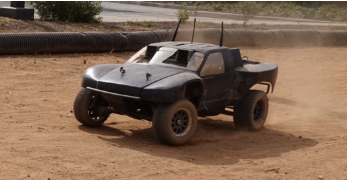
\includegraphics[height=.45\linewidth]{contents/chapt2/figs/IL_car.png}
        \caption[1/5 scale ground vehicle]{1/5 scale ground vehicle.}
        \label{fig:IL_car}
    \end{subfigure}
    \hfill
    \begin{subfigure}[htb!]{0.48\textwidth}
        \centering
        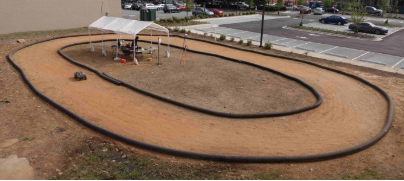
\includegraphics[height=.45\linewidth]{contents/chapt2/figs/IL_track.png}
        \caption[Oval gravel track]{Oval gravel track.}
        \label{fig:IL_track}
    \end{subfigure}
    \hfill
    \caption[The car and track used by Lee et al.]{The car and track used by Lee et al. \cite{lee2019}.}
\label{fig:lee_car_track}
\end{figure}


From these examples we see that imitation learning learning with neural networks is a powerful tool.
However, there are some weaknesses to the imitation learning technique:
The first is that the vehicle may encounter a scenario for which no expert training data was generated during training, in which case it is likely to take an incorrect action \cite{Osa_2018}.
This can happen because the learned policy affects the distribution of states that the vehicle encounters.
Since the learned policy differs slightly from the expert policy, the distribution of states that the imitation learned algorithm encounters is different to the training set.

%Furthermore, Wadekar et al. \cite{Wadekar2021} describe that the data collected by the expert must be curated so that the agent does not learn any undesirable behaviour. 

Perhaps the most undesirable characteristic of imitation learning is that it requires expert training data.
This makes it unsuitable for scenarios where expert training data is difficult to generate, as in cases where optimisation methods fail \cite{Fuchs2021}.
As such, we turn towards a method for training neural networks for control tasks that does not require expert training data.

\subsection{Reinforcement learning}
\label{sec:reinforcement_learning}

Reinforcement learning optimises a neural network policy to maximise a scalar reward signal through direct interaction with its environment \cite{Plaat_2022}. 
The benefits of using a neural network trained with reinforcement learning are the same as the imitation learning approach, i.e., less stringent sensor requirements and fast online execution time. 
However, the technique allows for more complex cost formulation than what is possible with even state of the art expert optimisation methods and negates the need for expert training data \cite{Fuchs2021}.
As such, it solves several of the drawbacks of the imitation learning algorithm.
We start our discussion on reinforcement learning approaches for autonomous racing by reviewing approaches aimed at driving cars in racing video games, then move towards approaches that solve more realistic driving scenarios.


\subsubsection*{Reinforcement learning applied to racing video games}
Although games allow assumptions to be made that would be unrealistic for physical vehicles (such as allowing collisions and the availability of opponents), they have played an important role in the advancement of reinforcement learning techniques applied to autonomous racing. 
These advancement include reward signal and neural network input design.
Furthermore, video game approaches have showcased state of the art results in a variety of scenarios, including single vehicle time trial and multi-vehicle racing.

Early works in reinforcement learning applied to autonomous racing, such as those by Perot et al. \cite{Perot2017} and Jaritz et al. \cite{Jaritz2018} were aimed at creating pixel-to-control strategies for World Rally Championship 6.
This means that images from the game screen were mapped to a control actions using a neural network. 
Both approaches succeed at controlling the vehicle, albeit with frequent track boundary collisions.
They also found that training a pixel-to-control algorithm is extremely inefficient, as both approaches took 80 million steps to train.

A more recent and state of the art approach is presented by Fuchs et al. \cite{Fuchs2021}, who created a model-free soft actor-critic (SAC) reinforcement learning agent that achieves time trial lap times on par with competitive e-sports drivers in the racing game Gran Turismo Sport.
Rather than use an image from the game screen as the input to the neural network, they carefully hand-craft a number of features. These are: 1) the vehicles velocity $\pmb{v}_t \in \mathbb{R}^3$, 2) acceleration $\pmb{\dot{v}}_t \in \mathbb{R}^3$, 3) distance measurements of $M$ rangefinders $\pmb{d}_t \in \mathbb{R}^M$, 4) the previous steering command $\delta_{t-1}$, 5) a binary flag indicating wall contact, and 6) $N$ sampled curvature measurements of the track centerline $\pmb{c}_t \in \mathbb{R}^N$.
These are important input features, as most other reinforcement learning approaches that do not utilise a pixel-to-control strategy use a selection of these features as input to their neural network.

Fuchs et al. \cite{Fuchs2021} also recognise that a reward given at the end of the race is too sparse for the agent to learn effectively. As such, they introduce a continuous reward signal that rewards progress while penalising the agent for making contact with the track boundary:
\begin{equation}
    r_t = r_{t}^{\text{progress}} - 
    \begin{cases}
    c_w \| \pmb{v}_t \| & \text{if in contact with wall} \\
    0 & \text{otherwise}
    \end{cases}
\end{equation}
where $c_w$ is a tuned constant.
Although their implementation remains in simulation, the effect of vehicle model inaccuracies by changing the parameters of the vehicle model between training and testing is noted. They find that increased tire friction causes the agent to steer more aggressively leading to brief contact with the inside wall. A decrease in tire friction causes the agent to take corners slightly wide resulting in contact with the outside.
However, it is not clear what degree of model inaccuracy results in collisions.

The previous approaches were aimed at solving time trial scenarios involving only one vehicle on the track.
However, the strength of reinforcement learning to allow agents to learn complex tasks is showcased best in multi-agent settings.
This is because when multiple vehicles are involved, the opponents behaviour must be taken into account to select an appropriate action.
However, these behavioral and environmental features may be too complex to be captured by classic optimisation approaches that need to assume perfect knowledge of the state of all vehicles.

Schwarting et al. \cite{Schwarting2021} showcase the strength of reinforcement learning to generate policies without perfect knowledge of the environment by training a model-based reinforcement learning algorithm to operate in a multi-agent setting where the opponent behaviour is initialy unknown.
Their solution learns a world-model that includes the opponent behaviour using a neural network, which is then then used to generate imagined gameplay experiences to train the agent on.

Another venture into the multi-agent setting is taken by Song et al. \cite{Song2021}, who extend the work from Fuchs et al. \cite{Fuchs2021}. 
They train an agent to overtake other vehicles in Gran Turismo Sport, as shown in Figure \ref{fig:RL_gran_turismo}.
key to their success is the use of curriculum learning, whereby the agent is trained to solve increasingly difficult tasks by adding components to both the environment and reward signal. 
This showcases the reinforcement learning algorithm's ability to adapt to changes in the environment.

\begin{figure}[htb!]
    \centering
    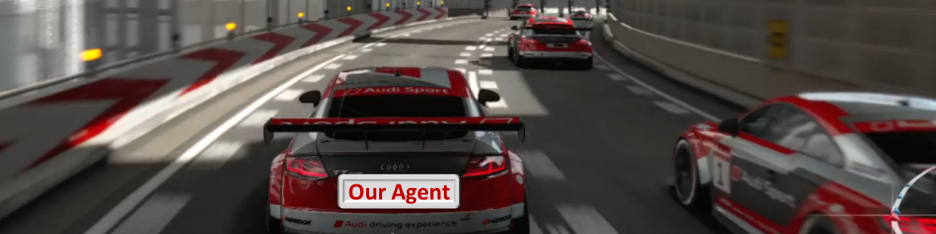
\includegraphics[width=0.8\textwidth]{contents/chapt2/figs/RL_gran_turismo.png}
    \caption[A reinforcement learning agent overtakes a vehicle in the racing game Gran Turismo Sport]{The reinforcement learning agent by Song et al. \cite{Song2021} overtakes a vehicle in the racing game Gran Turismo Sport.}
    \label{fig:RL_gran_turismo}
\end{figure}

%The agent is trained to race on its own before another vehicle is added to the simulation, and the reward signal is modified to encourage the agent to make progress relative to the other vehicle.
%This showcases the strength of reinforcement learning over optimisation methods: while optimisation algorithms rely on the convexification of cost functions, reinforcement learning agents can learn to solve difficult tasks from complex cost functions.



\subsubsection*{Reinforcement learning applied to realistic racing scenarios}

We now move away from now games and discuss research efforts that more directly address the sim2real gap and deployment onto physical cars.
There are a unique set of challenges to overcome while deploying reinforcement learning algorithms onto physical robots. 

A pertinent issue is that neural networks may select an unsafe action that leads to a collision.
Niu et al. \cite{Niu2020} address this by proposing a model-based safety controller that acts as a safeguard mechanism to prevent the agent from selecting unsafe actions.
Furthermore, they foresee that the safety module's reliance on an accurate vehicle model presents an issue. 
As such, a neural network is used to learn a vehicle model online that eventually replaces the initial assumed vehicle model.
This idea of improving a vehicle model after the vehicle is deployed is a commonplace sim2real practice.

Another issue that presents itself during physical deployment is that of control smoothness - reinforcement learning agents tend to select extreme control actions, such as steering fully to the left or right. 
Sudden control actions will induce excessive mechanical wear and cause the vehicle to exhibit dangerous behaviour.
Hsu et al. \cite{hsu2022} identify this issue and apply Conditioning for Action Policy Smoothness (CAPS) to smooth the control action of the vehicle.
Although Hsu et al. \cite{hsu2022} do not directly address model inaccuracies, their policy smoothing approach produces a conservative policy which is expected to increase performance and safety in settings where the model inaccuracies occur.
This is because a smoother policy results in less lateral and longitudinal acceleration and does not bring the vehicle as close to its handling limits as a jerkier policy.

Sim2real practices that directly address model inaccuracy are explored by Chisari et al. \cite{Chisari2021}, who made an agent policy robust to real-world transfer by training it with a slightly randomised vehicle model in simulation.
The agent policy is then refined by retraining the neural network after the physical vehicle is deployed.
This allows the reinforcement learning algorithms to achieve similar lap times but fewer track boundary collisions as an MPC controller.
Ivanov et al. \cite{Ivanov2020} take a similar approach to Chisari et al. \cite{Chisari2021} by training an agent with model randomisation, but are not able to achieve robustness to the sim2real transfer.

The final end-to-end approach we discuss is by Brunbauer et al. \cite{brunnbauer2021}, who demonstrate demonstrate the effectiveness of advanced model-based deep reinforcement learning agents in the real-world application of autonomous racing.
Brunnbauer et al. \cite{brunnbauer2021} deploy the model-based Dreamer reinforcement learning algorithm by Hafner et al. \cite{Hafner2019a} on a physical F1tenth vehicle.
Their algorithm learns an observation model which is used to predict agent-environment interactions.
It then learns a policy purely on imagined sequences using the observation model without interaction with the environment.
This results in safer deployment, as the agent can plan a sequence of actions ahead, rather than to select an action based purely on past experience.

From the literature reviewed, we see that there are many benefits to integrating neural networks into the driving pipeline.
These include learning from real-world data to improve the driving policy and vehicle dynamics model, shorter online execution time than optimisation methods, and a higher degree of flexibility in the algorithm input.
We also see that reinforcement learning is a viable approach to training a neural network within an end-to-end pipeline, as it circumvents the issue of relying on expert training data that imitation learning approaches suffer from.

However, wrapping the entirety of the driving task into one neural network has repercussions.
The driving behaviour of an end-to-end pipeline is difficult to design and interpret, leading to safety concerns.
Even slight errors in the control input can lead to very large errors in the trajectory, resulting in catastrophe.
Furthermore, the standard end-to-end pipeline is not particularly robust to model inaccuracies that occur when deploying driving algorithms onto physical vehicles, unless the neural network is trained using a set of sim2real best practices.
A summary of the end-to-end reinforcement learning approaches discussed is shown in Table \ref{table:autonomous_racing_rl_summary}.

%Conclusion:
%RL techniques over MPC and IL
%Challenges to vehicle behaviour
%Challenges with sim2real transfer due to model mismatch
%Classical approaches absorb uncertainty using a controller.
%Presents a question to system architecture design: integrating a neural network into the classical pipeline.


\section{Partial end-to-end pipeline}
\label{sec:partial_end_to_end}


%Wrapping the entirety of the driving task into one neural network has repercussions.
%As the neural network needs to learn all three high level tasks from the classical pipeline (perception, planning and control), it can %Betz et al. and \cite{Weiss2020} et al. \cite{Betz2021} argue that it would be simpler to learn only one task from the classic pipeline.
%Furthermore, Weiss et al. \cite{Weiss2020} argue that even though end-to-end methods perform well on validation data, that does not mean that the method contains a useful driving strategy that can perform well in an actual driving test.
%This is because end-to-end methods fail to capture how expert drivers behave.
%Expert drivers do not select only the control action at the current time step based on their current vehicle state, but instead plan out a trajectory. 
%They then execute control commands to achieve that trajectory.
%Furthermore, slight errors in the control input can lead to very large errors in the trajectory, resulting in catastrophe.

We now consider the approach to designing autonomous driving algorithms that synthesises the classic and end-to-end pipelines. 
In the partial end-to-end approach, the modular structure of the classic pipeline is utilised.
However, rather than using techniques associated with the classic pipeline for implementing individual modules, the function of a module is learned using a neural network.
Approaches following this driving algorithm architecture may benefit from the structure the classic pipeline and the use of neural networks from the end-to-end pipeline.

There are two possible architectures within the partial end-to-end pipeline: either the controller or the trajectory planner is learned using a neural network. 
These two architectures are shown in Figure \ref{fig:pete_learned_control} and \ref{fig:pete_learned_control}, respectively.
We now give attention to research efforts into both architectures within the partial end-to-end pipeline.


%\begin{landscape}
    %\newcolumntype{a}{>{\hsize=1\hsize \centering\arraybackslash}X}
\newcolumntype{d}{>{\hsize=.5\hsize \centering\arraybackslash}X}
\newcolumntype{e}{>{\hsize=2\hsize \centering\arraybackslash}X}


\begin{table}[h]
\centering
\begin{tabularx}{21cm}{|a|d|d|d|d|e|}
    
    \hline
    \small \textbf{Name} & \small \textbf{Model-based} & \small \textbf{Multi-agent} & \small \textbf{Input} & \small \textbf{Physical vehicle} & \small \textbf{sim2real approach} \\
    \hline
    \small Schwarting et al. \cite{Schwarting2021} & \checkmark & \checkmark & \small game image & & - \\
    \hline
    \small Brunnbauer et al. \cite{brunnbauer2021} & \checkmark & & \small features & \checkmark & - \\
    \hline
    \small Perot et al. \cite{Perot2017} & & & \small game image & & - \\
    \hline
    \small Jaritz et al.  \cite{Jaritz2018} & & & \small game image & & - \\
    \hline 
    \small Fuchs et al. \cite{Fuchs2021} & & & \small features & & \small Test effects of model inaccuracy in simulation \\
    \hline
    \small Remonda et al. \cite{Remonda2021} & & & \small features & \checkmark & - \\
    \hline 
    \small Song et al. \cite{Song2021} & & \checkmark & \small features & & - \\
    \hline
    \small Niu et al. \cite{Niu2020} & & & \small features & & \small Safety module based on learned vehicle model prevents agent from selecting unsafe actions. \\
    \hline
    \small Chisari et al. \cite{Chisari2021} & & & \small features & \checkmark & \small Parameter randomisation while training, policy refinement after deployment \\
    \hline
    \small Ivanov et al. \cite{Ivanov2020} & & & \small features & \checkmark & \small Parameter randomisation while training \\
    \hline
    \small Hsu et al. \cite{hsu2022} & & & \small image & \checkmark & \small Control action smoothing \\
    \hline

\end{tabularx}
\caption[A summary of end-to-end reinforcement learning approaches for autonomous racing]{A summary of end-to-end reinforcement learning approaches for autonomous racing.}
\label{table:autonomous_racing_rl_summary}
\end{table} 

    %\footnote{The absence of a tick in the model-based, multi-agent , and physical vehicle columns indicate that the approach was model%-free, single-agent and simulation only, respectively. \label{footnote_1}}
%\end{landscape}

\begin{landscape}
    \newcolumntype{R}{>{\raggedleft\arraybackslash}p{2.7cm}}
\newcolumntype{M}{>{\centering\arraybackslash}p{1.8cm}}
\newcolumntype{N}{>{\centering\arraybackslash}p{2.2cm}}
\newcolumntype{Y}{>{\centering\arraybackslash}p{1cm}}
\newcolumntype{L}{>{\raggedright\arraybackslash}p{7cm}}


\begin{table}[htb!]
\centering
\renewcommand{\arraystretch}{1.5}
%\resizebox{\textwidth}{!}{
\begin{tabularx}{0.9\textwidth}{R Y M L}
    \hline
    \small \textbf{Author(s)} & \small \textbf{Year} & \small \textbf{Physical \mbox{vehicle}} & \small \textbf{Sim2real research contribution} \\
    \hline
   
    \small Jaritz et al. \cite{Jaritz2018} & \small 2018 & & - \\

    \small Perot et al. \cite{Perot2017} & \small  2017 & & - \\

    \small Fuchs et al. \cite{Fuchs2021} & \small 2021 & & \small Test effects of model inaccuracy in simulation. \\

    \small Song et al. \cite{Fuchs2021} & \small 2021 & & - \\

    \small Wurman et al. \cite{Wurman2022} & \small 2021 & & - \\

    \small Cai et al. \cite{Cai2020} & \small 2021 & & - \\

    \small Niu et al. \cite{Niu2020} & \small 2020 & & \small Safety module based on learned vehicle model prevents agent from selecting unsafe actions. \\
    
    \small Brunnbauer et al. \cite{brunnbauer2021} & \small 2021 & F1tenth & - \\

    \small Hsu et al. \cite{hsu2022} & \small 2022 & F1tenth & \small Domain randomisation while training. Control action smoothing. \\

    \small Ivanov et al. \cite{Ivanov2020} & \small 2020 & F1tenth & \small Domain randomisation while training. \\

    \small Chisari et al. \cite{Chisari2021} & \small 2021 & $1:43$ scale cars & \small Domain randomisation while training, policy refinement after deployment. Control action smoothing.\\

    \hline

\end{tabularx}
%}
\caption[A summary of end-to-end reinforcement learning approaches for autonomous racing]{A summary of end-to-end reinforcement learning approaches for autonomous racing. }
\label{table:autonomous_racing_rl_summary}
\end{table} 

\end{landscape}


\begin{figure}[htb!]
    \centering
    \begin{subfigure}[htb!]{\textwidth}
        \centering
        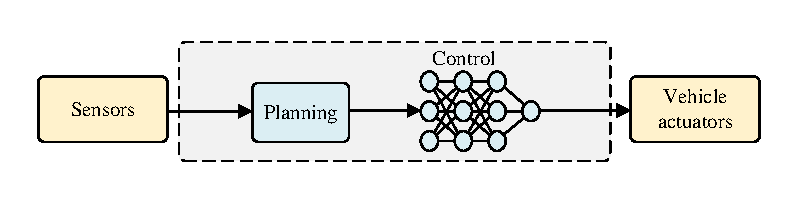
\includegraphics{contents/chapt2/figs/partial_end_to_end_pipeline_learned_control.pdf}
         \caption[The partial end-to-end pipeline with a learned controller]{The partial end-to-end pipeline with a learned controller.}
        \label{fig:pete_learned_control}
    \end{subfigure}
    \hfill
    \begin{subfigure}[htb!]{\textwidth}
        \centering
        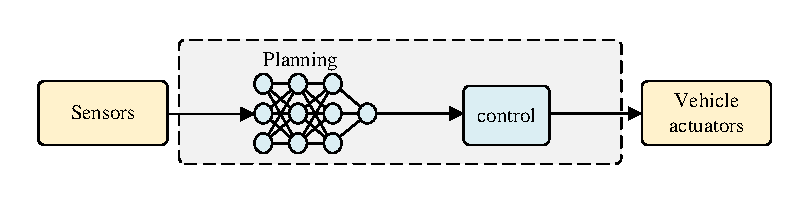
\includegraphics{contents/chapt2/figs/partial_end_to_end_pipeline_learned_trajecory_planning.pdf}
        \caption[The partial end-to-end pipeline with a learned trajectory planner]{The partial end-to-end pipeline with a learned trajectory planner.}
        \label{fig:pete_learned_trajectory_planning}
    \end{subfigure}
\caption[Configurations of the partial end-to-end pipeline]{The two configurations of the partial end-to-end pipeline.}
\label{fig:pete}
\end{figure}


\subsection{Learned controller}
\label{sec:learned_controller}

In the literature reviewed, there were two attempts at creating a partial end-to-end pipeline whereby the controller function is learned by a neural network.
The first approach we look at is by Evans et al. \cite{Evans2021b}, who combined a reinforcement learning agent with a pure pursuit path follower that tracks a global path.
By modifying control commands from the controller, the agent is able to avoid randomly placed obstacles.
However, a kinetic bicycle model that does not account for tire slipping was used.
As such, the performance of their system under more realistic racing conditions is unknown.

The other was by Ghignone et al. \cite{Ghignone2022}, who replaced the controller with a reinforcement learning agent.
Their agent was trained with varying tire friction coefficients to generalise to different model parameters.
It outperformed both an the MPC controller and end-to-end agent in terms of track boundary collisions by a large margin under model mismatch conditions.
However, Ghignone et al. \cite{Ghignone2022} do not describe the exact parameter values that result in this performance difference.
Furthermore, their approach does not include a local planner.
If the classic structure were adhered to, the neural network controller will need to be combined with a local planner from the classical pipeline. 
As such, approaches following this architecture will suffer from the drawbacks of those local planners, as described in Section \ref{sec:trajectory_planning}.


\subsection{Learned Trajectory planner}
\label{sec:learned_planner}
We now discuss approaches where the local trajectory planning task is learned by a neural network.
The learned trajectory planner is used in conjunction with a classic controller, as shown in Figure \ref{fig:pete_learned_trajectory_planning}. 
This architecture may benefit from the use of classic controllers which absorb uncertainty in the system by decreasing the error between the actual and planned trajectory in a predictable manner.
As such, it may be a viable technique to combat the degradation in performance due to model uncertainty that end-to-end approaches suffer from. 
Furthermore, it avoids the pitfalls of the trajectory optimisation techniques associated with the classic pipeline.

Weiss et al. \cite{Weiss2020a} trained an imitation learning agent to generate a local path as a bezier curve.
A pure pursuit controller is used to ensure that the vehicle tracks this path.
A similar approach is taken by Capo et al. \cite{Capo2020}, except that a reinforcement learning agent outputs only a single point in front of the vehicle, which is tracked using low-level logic.
Both of these approaches outperformed end-to-end approaches in terms of distance raced before colliding with track boundaries, and generalisation across different tracks. However, they do not take model uncertainty into account.
A summary of the partial end-to-end techniques in literature is presented in Table \ref{table:autonomous_racing_partial_end_to_end_summary}.
%All partial end-to-end pipeline results indicate that the partial end-to-end pipeline outperforms the end-to-end pipeline.

\newcolumntype{R}{>{\raggedleft\arraybackslash}p{2.7cm}}
\newcolumntype{M}{>{\centering\arraybackslash}p{1.8cm}}
\newcolumntype{N}{>{\centering\arraybackslash}p{2.2cm}}
\newcolumntype{Y}{>{\centering\arraybackslash}p{1cm}}
\newcolumntype{L}{>{\raggedright\arraybackslash}p{4.5cm}}

\begin{table}[htb!]
\centering
\small
\renewcommand{\arraystretch}{1.1}
\begin{tabularx}{0.9\textwidth}{RYMNL}
    \hline
    \small \textbf{Author(s)} &  \small \textbf{Year} & \small \textbf{Learning method} & \small \textbf{Learned component} & \small \textbf{sim2real approach} \\
    \hline
    \small Weiss and Behl \cite{Weiss2020, Weiss2020a, Weiss2022} & \small $2020$ & \small IL & \small Planner  & - \\
    \small Capo et al. \cite{Capo2020} & \small $2022$ & \small RL &  \small Planner & - \\
    % \small Mahmoud et al. \cite{Mahmoud2020} & \small $2020$ & \small RL & \checkmark & & - \\
    \small Evans et al. \cite{Evans2021b} & \small $2021$ & \small RL &  \small Controller & - \\
    \small Ghignone et al. \cite{Ghignone2022} & \small $2022$ & \small RL &  \small Controller  & \small Randomise vehicle model parameters while training \\
    \hline
\end{tabularx}
\caption[A summary of partial end-to-end approaches for autonomous racing]{A summary of partial end-to-end approaches for autonomous racing.}
\label{table:autonomous_racing_partial_end_to_end_summary}
\end{table} 


\section{F1Tenth racing}\label{sec:f1tenth}

F1Tenth is an autonomous racing competition that allows teams to compete with a standardised set of hardware and rules.
The organisers of the competition provide specifications for the vehicle, such as the chassis, onboard computer and sensors.
Furthermore, to aid the development process, a vehicle simulator is provided. 
The track is known prior to the races, and its boundaries are built from LiDAR perceivable material.
The standardisation of the vehicles and LiDAR perceivable track boundaries shifts the research focus towards racing algorithm design.
The hardware and software support that the F1Tenth platform provides makes it an ideal test-bed for autonomous vehicle development \cite{f1tenth}.

The competition comprises two stages, a time trial event and a head-to-head race.
In time trial, the goal is to drive around the track as fast as possible without any other vehicles on the track, whereas in head-to-head racing there are two vehicles on the track at the same time, as shown in Figure \ref{fig:f1tenth_prague}.
For both of the stages of the event, the cars must navigate using only onboard sensors and computers. 
This introduces a limitation on the computational expense of the algorithms that teams can deploy \cite{f1tenth}.

\begin{figure}[htb!]
    \centering
    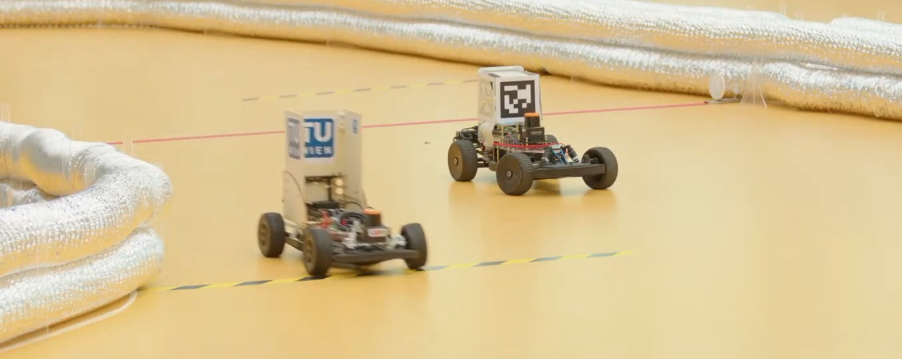
\includegraphics[width=\textwidth*7/10]{contents/chapt2/figs/f1tenth_prague_1.png}
    \caption[Two F1Tenth cars racing head-to-head]{Two F1Tenth cars race head-to-head at the International Conference on Intelligent Robots and Systems (IROS) 2021 event \cite{f1tenth}.}
    \label{fig:f1tenth_prague}
\end{figure}


\section{Research Gaps and Expected Contributions}
\label{research_gap}
Having explored current solutions to developing autonomous driving architectures, we identify a few trends in the literature.
Research efforts into utilising machine learning for decision making in autonomous racing have been largely limited to end-to-end systems. 
Within these learning (i.e., end-to-end) approaches, reinforcement learning is an especially attractive method for training the neural network because it negates the need for expert training data.

Although the end-to-end approach has shown promising results in simulation, deployment onto hardware remains a challenge.
Aside from the safety concern of wrapping the entire driving task into one neural network, the degradation in performance due to model inaccuracy while deploying agents onto physical vehicles is an issue.
Although some approaches do combat sensitivity towards model inaccuracy in end-to-end systems by randomising model parameters during training or refining the vehicle model after deployment, these techniques do not guarantee the safety of the vehicle, as end-to-end systems still crash after physical deployment.
Furthermore, the effect of this model inaccuracy is not well quantified.

There have been only a few attempts at integrating machine learning into the modular structure of the classical pipeline, as in the partial end-to-end pipeline.
These research efforts have shown promise, with several results indicating that partial end-to-end outperforms end-to-end.
This is because partial end-to-end systems may benefit from the advantages that both the classical and end-to-end offer: the structure of the end-to-end pipeline eases development, while the learning methods from end-to-end approaches provide flexibility.

In particular, we have identified the partial end-to-end approach whereby a neural network trajectory planner is used in conjunction with a classic controller as a suitable method to combat the sensitivity towards model inaccuracy that current learning systems experience.
This is because controllers are used to absorb uncertainty within the classic pipeline.
However, whether this approach will actually result in a performance benefit over purely end-to-end systems under model-mismatch conditions is not explored in literature and remains an open question - one which we aim to answer through this project.
We conclude this section by repeating the literature taxonomy in Figure \ref{fig:literature_taxonomy_1}, but with the leaf nodes showing research papers we reviewed. We also indicate where our approach fits into the taxonomy.

\begin{figure}[h]
    \centering
    \input contents/chapt2/figs/literature_taxonomy_articles.tex
    \caption[A taxonomy of the autonomous racing literature with articles]{A taxonomy of the autonomous racing. The blue leaf nodes reference the articles relevant to their description.}
    \label{fig:literature_taxonomy_1}
\end{figure}

